\chapter{Controller design}
Controller design of Attitude controller is based upon the simulink model, described in Chapter \ref{ch:6}. Hovering the quadcopter is done with an inner-(rotational rate) and outer-loop (attitude). Regarding position control uses these two loops as well and adds two extra loops; position and velocity feedback. All loops are explained in detail below.\\

\section{Angle control}
The angle control which is done with feedback of angular position and angular velocity. The inner loop is tuned first while using multiple feedback loops, which is the rotational rate loop. $p$,$q$ and $r$ (roll-, pitch-, yaw-rate) are tuned seperately and checked if functional in the combined system. The tuning for roll is shown in Figure \ref{fig:rollratestep}.

\begin{figure}[H]
\centering
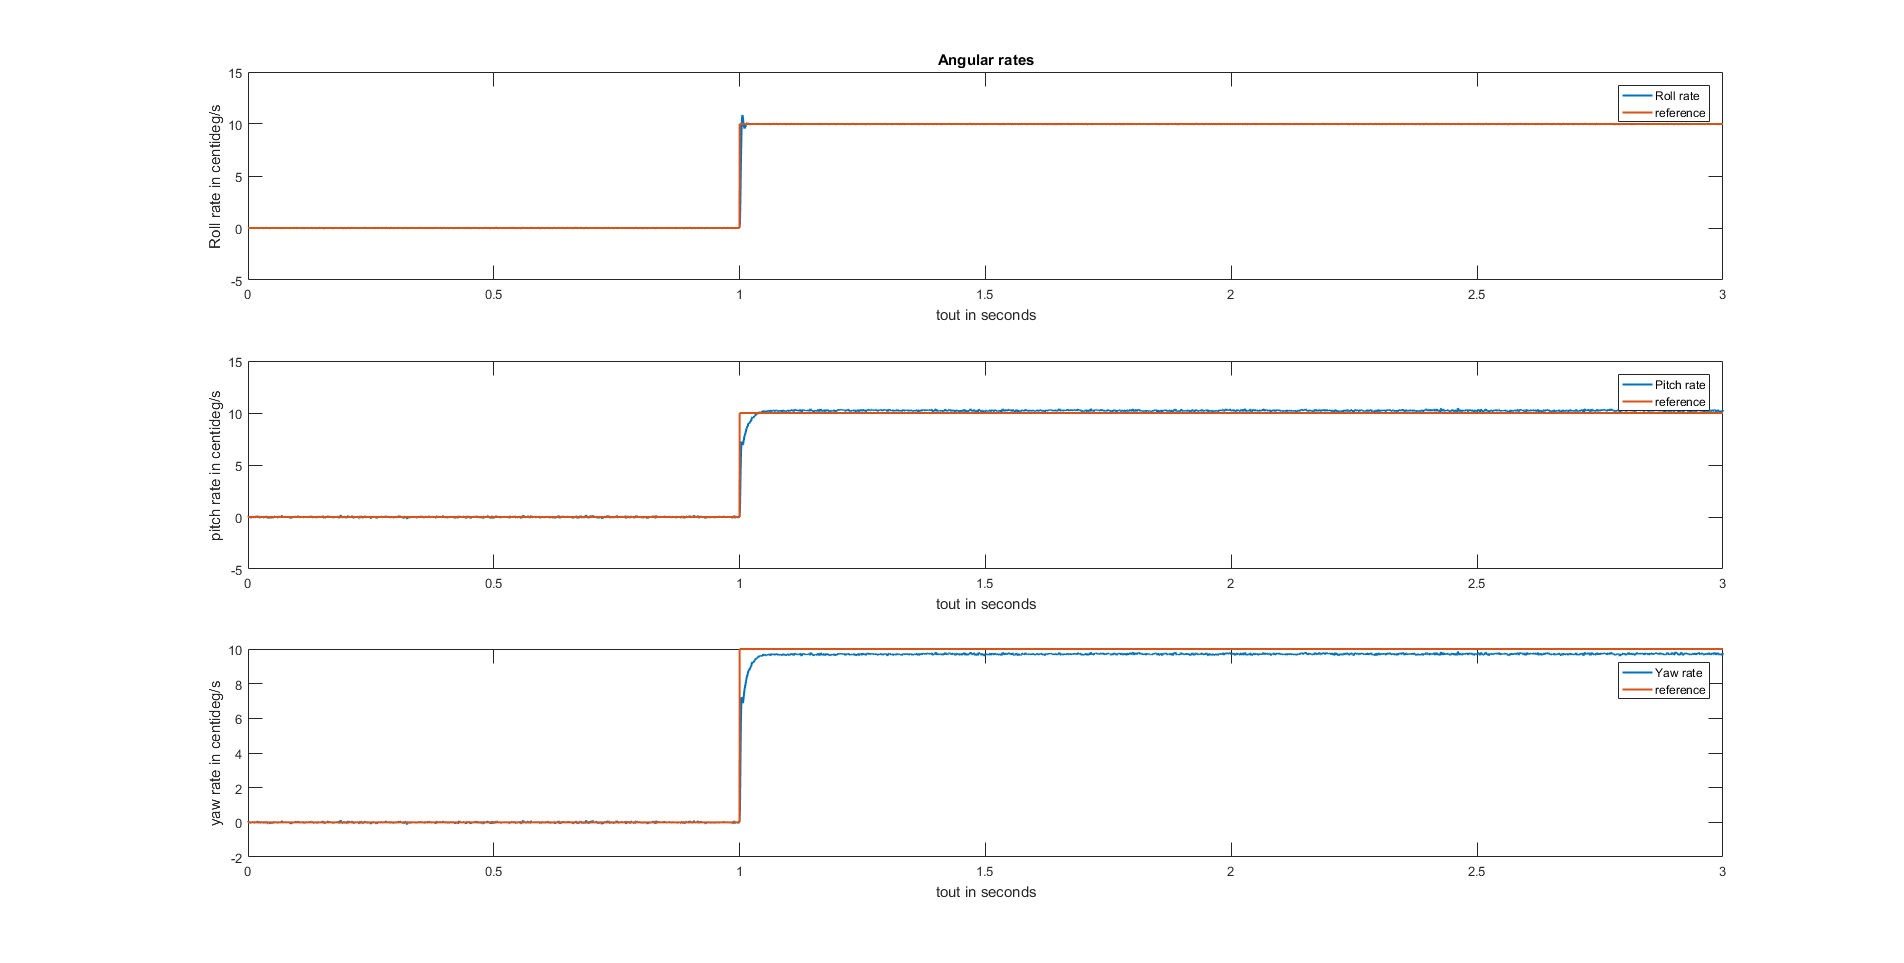
\includegraphics[width=0.8\textwidth]{RateControllerTuning.png}
\caption{Step response in rotational rate showing that the tracking controller works proper.}
\label{fig:RateControllerTuning}
\end{figure}

\textcolor{red}{nieuw plotje maken (netter)}
Firstly P-action is added to increase the speed of the system, D-action to prevent overshoot and an extra I-action to decrease the overall error. The tuned controller shows that the rotational rate follows the reference nicely. Thereafter is the attitude controlled. Since inner loop is already controlled, only P-action is needed in attitude to obtain good tracking. Increasing the gain is however shows that the attitude introduces an overshoot. This can be solved by adding a D-action in the attitude, or by increasing the gain in the rotational rate controller, which is also derivative action for the attitude. After retuning, the result is visible in Figure \ref{fig:AttitudeControl}.

\begin{figure}[H]
\centering
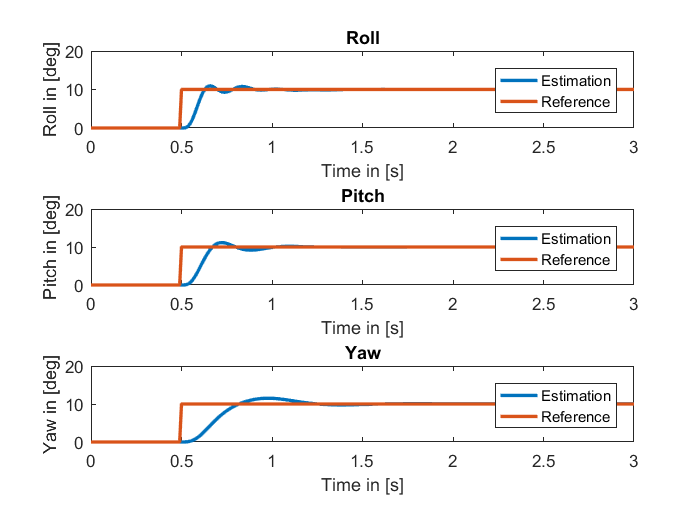
\includegraphics[width=0.8\textwidth]{Attitudestepresponse.png}
\caption{Step response in the three angles showing that the tracking controllers works proper.}
\label{fig:AttitudeControl}
\end{figure}

\textcolor{red}{Misschien nog een figuur bij stoppen die de rate laat zien bij een step response in attitude.}

Note that in case of position control, the controller of the attitude has to be tuned at another point in the control scheme, but will be tuned with the same method.

\section{Position Control}
\textcolor{red}{Hier plaatjes van horizontal velocity (PID?) en  horizontal position(P?)}
\textcolor{red}{plaatje van desired angle en hoe die hem trackt}
\textcolor{red}{Plaatje van altitude control.}


\section{Compensating Near-wall effect}
Attitude dynamics of rotational rate is needed to be described to create a disturbance observer. These can be discribed in the same way as in [3 hier profs paper] described in the set equations of \ref{eq:attdyn}

\begin{equation} \label{eq:attdyn}
\begin{aligned}
\dot{x}_1 &= x_2 \\
\dot{x}_2 &= F(t)+bu \\
y 		  &=x_1 
\end{aligned}
\end{equation}

With $x_1$ and $x_2$ as rotational-rate and -acceleration, $F(t)$ as external disturbance, $b$ and $u$ are statematrix and input. Since $F(t)$ is not known, because of fluctions and dependencies of wall gap. Consequently, $F(t)$ is considered state $x_3$ and let $\dot{x}_3 = G(t)$. The equations of \ref{eq:attdyn} become \ref{eq:attdyn2}

\begin{equation} \label{eq:attdyn2}
\begin{aligned}
\dot{x}_1 &= x_2 \\
\dot{x}_2 &= x_3+bu \\
\dot{x}_3 &= G(t)
y &=x_1 
\end{aligned}
\end{equation}

It is possible to create an extended state observer now to estimate the states $x_1$ and $x_2$ and disturbance $x_3$, since the dynamics are now in canonical form and is therefore observable. Examples of a linear observer is shown in Equation \ref{eq:attobs}

\begin{equation} \label{eq:attobs}
\begin{aligned}
\dot{z}_1 &=z_2-L_1e +bu\\
\dot{z}_2 &= -L_2e
\end{aligned}
\end{equation}
With 
\begin{equation}
e=y-z_1
\end{equation}

With $z$ as the observed states and disturbance and $L$ as the observer gains. The choice of $L$ is created by the designer, which is explained in further detail lateron. Discretizing the system gives 

\begin{equation}
\begin{aligned}
z_1(k+1) &= z_1(k)+T_s\left(z_3(k)+bu(k)\right) - \beta_{01}e(k)\\
z_2(k+1) &= z_2(k)-\beta_{02}e(k) 
\end{aligned}
\end{equation}
with 
\begin{equation}
\begin{aligned}
e(k) = y(k)-z_1(k)
\end{aligned}
\end{equation}

These final equations are used in the model which is visible in Figure \ref{fig:DOBCscheme}.

\begin{figure}[H]
\centering
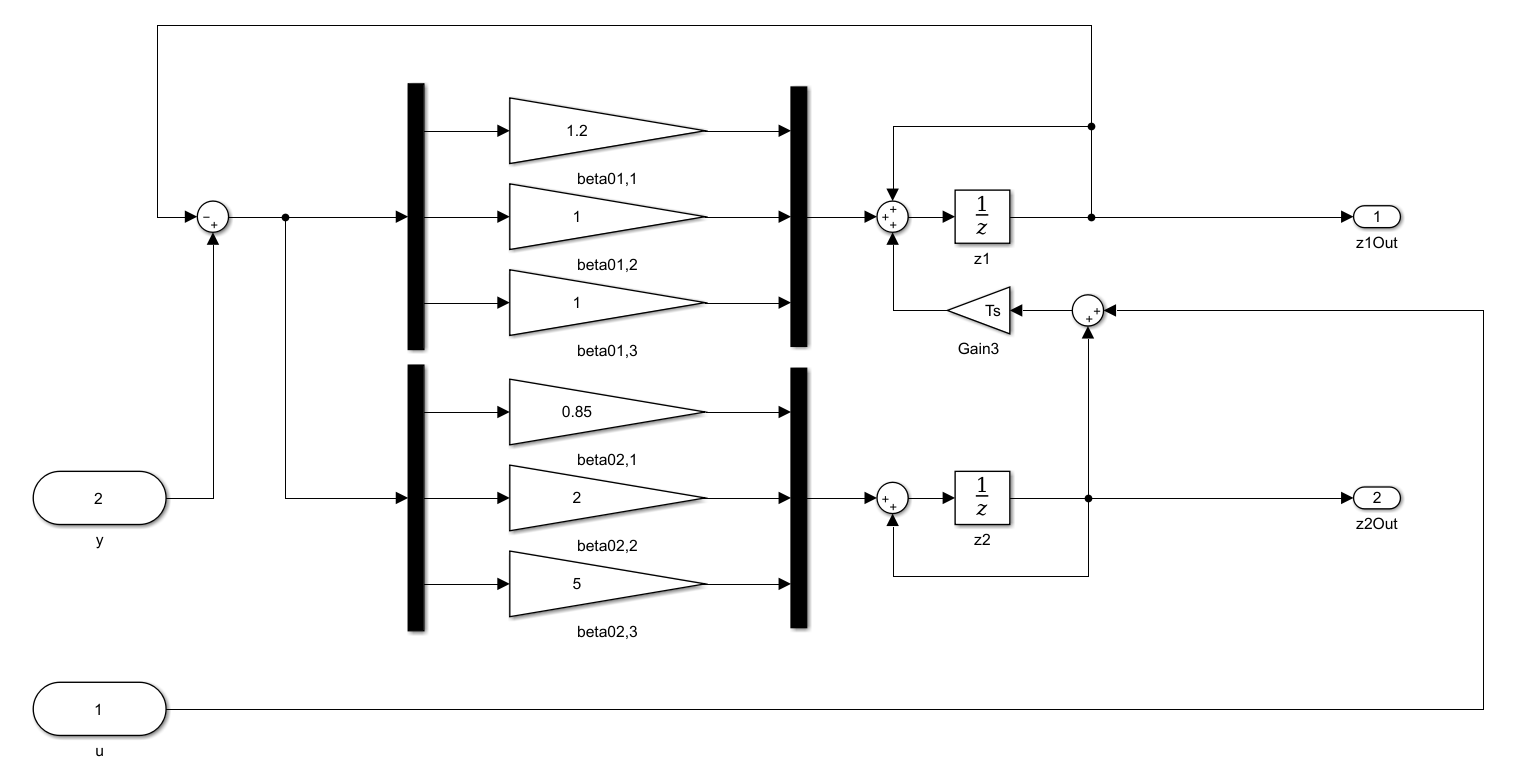
\includegraphics[width=0.8\textwidth]{DOBCscheme.png}
\caption{Control scheme of DOBC with $y$ the output, $u$ the input, $z_{1out}$ estimated rotational rate and $z_{2out}$ the estimated disturbance.}
\label{fig:DOBCscheme}
\end{figure}

